\chapter{Megvalósítás}\label{ch:MEGVALOSITAS}
\begin{osszefoglal}
	A dolgozat tárgyát képező projekt egy EV3 készletből épített kétkerekű egyensúlyozó robot irányítását valósítja meg hálózaton keresztül, telefonos alkalmazás segítségével. E fejezetben bemutatásra kerülnek a megvalósítás során felmerült problémák, ezek megoldása és a felhasznált technológiák.
\end{osszefoglal}

\section{EV3 programozása}\label{sec:MEGVALOSITAS:lejos}
A LEGO MINDSTORMS kifejlesztett egy programozási környezetet, mely célja, hogy a megépített robotot különböző funkcionalitásokkal lehessen felruházni. E környezet lehetővé teszi a kisebb korosztály számára is a robotok programozását. Különböző grafikus elemekből úgynevezett blokkokból épül fel a program, amely USB-n keresztül kitelepíthető az EV3 vezérlőegységen futó LEGO MINDSTORMS által fejlesztett firmware.
Az előbb említett programozási környezet nem alkalmas komplexebb problémák megoldására. Ezért több firmware-t is kifejlesztettek melyek magas szintű programozási nyelvek használatát támogatják, ilyen a ROBOTC\footnote{\href {http://www.robotc.net}{http://www.robotc.net}} Carnegie Mellon egyetem fejlesztette ki, amely támogatja a C programozást illetve megemlíteném még a Debian\footnote{\href{https://www.debian.org/}{https://www.debian.org/}} által kifejlesztett ev3dev-at \footnote{\href{http://www.ev3dev.org/}{http://www.ev3dev.org/}} amely a szkript nyelveket támogatja (Phyton, NodeJS, Ruby) . Esetünkben a leJOS firmware-t használjuk.

A leJOS firmware-t José Solórzano hozta létre 1999 végén és azóta is folyamatosan fejlesztik. Linux alapú, nyílt forráskódú, magába foglalja a JVM-t (Java virtual machine), a neve is rámutat a Java programozhatóságra JOS(Java Operating System). Futtatási környezetet biztosít a Java programozóknak, támogatja az objektum orientált programozást. Mindezek lehetővé teszik a socket alapú komunikációt, szinkronizálhatóságot, szálak alkalmazását és Java típusok használatát.

Az EV3 vezérlőegységen található négy bemeneti (S1, S2, S3, S4) illetve négy kimeneti (A, B, C, D) port. A bemeneti portok esetén a szenzorok csatlakoztathatjuk valamint a kimeneti portok esetén a motorokat. A leJOS hozzáférést biztosít ezekhez a portokhoz. Amint látható a \ref{motorPort} illetve a \ref{gyroPort} ábrán explicit megkel adjuk, hogy milyen porton található a motor illetve a szenzor. Motorok esetén importálnunk kell \texttt{lejos.hardware.port.MotorPort} csomagot és így elérjük a \texttt{MotorPort} interface-t. Szenzorok esetén is hasonló az eljárás, azzal a különbséggel hogy ebben az esetben a \texttt{lejos.hardware.port.SensorPort} csomagot kell importáljuk a \texttt{SenzorPort} inteface eléréséhez.

A motorok illetve a szenzorok példányosításához szükséges megadni a motor vagy szenzor megfelelő portját. A leJOS elrejti a szenzorok implementációját, lehetővé téve a magas szintű absztrakció használatát.

A motorok példányosítása esetén az objektum típusának kiválasztása a motor típusától függ és a mód kiválasztásától. A motor típusát meghatározza a mérete(nagy illetve közepes motorok). Módok kiválasztása esetén lehetőségünk van szabályzott mód (\ref{motorRegMod} ábrán látható) illetve nem szabályzott mód  (\ref{motorUnregMod} ábrán látható) közti választására. A motorok nem szabályzott módjának típushierarchiája megtekinthető a \ref{fig:unregMotorHierhachia} ábrán illetve a szabályzott mód a \ref{fig:regMotorHierhachia} ábrán.

\begin{figure}[!htb]
	\centering
	\minipage{0.5\textwidth}
	\pgfimage[width=0.9\linewidth]{images/unregMotor}
	\captionsetup{justification=centering,margin=1.5cm}
	\caption{Nem szabályozott mód szervomotorok típushierarchia}
	\label{fig:unregMotorHierhachia}
	\endminipage
	\minipage{0.5\textwidth}
	\pgfimage[width=0.9\linewidth]{images/regMotor}
	\captionsetup{margin=1.5cm}
	\caption{Szabályozott mód nagy szervomotorok típushierarchia}
	\label{fig:regMotorHierhachia}
	\endminipage
\end{figure}
 
 A szenzorok esetén az objektum példányosítását követően választjuk ki a lehetséges módok közül a nekünk megfelelőt. Ehhez szükségünk van a \texttt{SensorMode} objektumra amely a későbbiekben biztosítja e mód metódusait. A szenzoroknak megfelelő objektum esetén a motorokkal ellentétbe mindegyik származtatja a \texttt{UARTSensor} osztály, a \ref{fig:gyroHierhachia} ábrán látható.

\begin{figure}[!htb]
	\centering
	\pgfimage[width=0.5\linewidth]{images/gyroSenzor}
	\caption{Giroszkóp szenzor típushierarchia}
	\label{fig:gyroHierhachia}
\end{figure}


A \ref{gyroRateMod} és a \ref{gyroAngleMod} ábrákon látható a leJOS firmware által biztosított két mód, a giroszkóp szenzor használatához. A \texttt{rate} mód a szögsebességet méri, amelyet szög/másodperce -ben kapunk meg. Esetünkben szükségünk van a robot dőlési szögére is, amelyet a \ref{egyensulySubSec} alfejezetben látható \ref{szog} képlet segítségével  kiszámítunk. A \ref{gyroRateMod} ábrán látható az előbb említett mód kiválasztása és ezt követően a mintavételezés, melynek eredménye a \texttt{sample} tömb első eleme lesz. Használható \texttt{angle} módban is, amely \ref{gyroAngleMod} ábrán látható. E mód a szenzor kezdő orientációjához képest mér. Mintavételezés hasonlóan történik, mint az előbb említett módnál, annyi különbséggel hogy ez esetben szöget mér a kezdő pozíciójához képest. Mindkét mód esetében a \texttt{reset} metódus hívással újra kalibrálhatjuk a szenzort.

\begin{lstlisting}[label=gyroRateMod, caption= Giroszkóp szenzor \texttt{rate} mód használata, language=Java]

float[] sample = new float[1];
EV3GyroSensor gyroSensor =  new EV3GyroSensor(SensorPort.S2);

SampleProvider gyroMode = gyroSensor.getRateMode();

gyro.fetchSample(sample, 0);

\end{lstlisting}

\begin{lstlisting}[label=gyroAngleMod, caption= Giroszkóp szenzor \texttt{angle} mód használata, language=Java]

float[] sample = new float[1];
EV3GyroSensor gyroSensor =  new EV3GyroSensor(SensorPort.S2);

SampleProvider gyroMode = gyroSensor.getAngleMode();

gyro.fetchSample(sample, 0);

\end{lstlisting}

A nagy motorok esetében is két módot biztosít a leJOS firmware, amelyek a \ref{motorUnregMod} és \ref{motorRegMod} ábrán láthatóak. Rendre értelemszerűen a nem szabályzott és a szabályzott módok. 

A motor nem szabályzott mód (\ref{motorUnregMod} ábra) használata esetén az irányítást a \texttt{setPower} metódus hívással valósítjuk meg, amelynek -100 és 100 közötti értéket adhatunk át. Az átadott érték határozza meg, hogy mekkora erőt fejtsen ki a motor, ha az átadott érték pozitív akkor előre forog illetve ha negatív akkor hátra. A \texttt{resetTachoCount} valamint \texttt{getTachoCount} metódusokkal kezeljük a motorban levő forgás mérő szenzort, melynek számlálójának értékét lekérhetjük vagy lenullázhatjuk. Esetünkbe szükséges a pozíció illetve a sebesség meghatározása, e megvalósításához szükséges az előbb említett metódus által lekérni a két motor fordulat számát, amelyeket átlagoljuk, ezáltal kiszűrjük a szenzor mérésénél keletkezett zajokat. Az így megkapott értéket átalakítjuk szögbe majd kiszámítjuk a \ref{egyensulySubSec} alfejezetben megjelenő (\ref{sebesseg}) és (\ref{pozicio}) képletek segítségével. A \texttt{stop} metódus hívása esetén a motor blokkolt állapotba kerül.    

A motor szabályzott mód (\ref{motorRegMod} ábra) esetén némely funkcionalitás eltér az előbb említett módhoz képest. Ez esetben a motor sebessége fok/másodperc-ben megadható a \texttt{setSpeed} metódus által. A forgás sebessége függ az akkumulátor töltöttségi szintjétől, a maximális sebessége 740 fok/másodperc. A \texttt{rotate} metódussal adjuk meg, hogy hány fokot forduljon a motor. E metódusnak két változata van. Megadhatjuk csak a fokot vagy egy logikai értékkel megadható, hogy miután elérte az adott forgási fokot magától megálljon a motor. Ez esetben ha forgás közben meghívódik egy másik metódus, mely parancsot ad a motornak akkor az előbb kiadott utasítás végrehajtása leáll. A \texttt{waitComplete} metódussal lehetőség van, hogy bevárja a forgás befejezését, tehát addig vár míg végrehajtja a motor az azelőtt kapott utasítást. Az előbb említett mód esetén a pozíciót és a sebességet ki kellet számolni. Ez esetben lehetőség van ezen értékek lekérésére a \texttt{getPosition} és \texttt{getSpeed} metódusok által.

Esetünkben lényeges különbség a két mód között, hogy a szabályzott mód esetén jóval lassabb a motorok reagálási ideje mint a nem szabályzott mód esetén. E mellet a szabályzott mód használatakor ha kiadunk egy utasítást akkor kell figyeljünk, hogy utána ne adjunk olyan más utasítást amely miatt az előzőt leállítaná.

\begin{lstlisting}[label=motorUnregMod, caption=  A nagy motor \texttt{unregulated} mód használata, language=Java]

EncoderMotor motor = new UnregulatedMotor(MotorPort.A)

motor.resetTachoCount();
motor.setPower(40);

int tacho = motor.getTachoCount();

motor.stop();

\end{lstlisting}

\begin{lstlisting}[label=motorRegMod, caption= A nagy motor \texttt{regulated} mód használata, language=Java]

RegulatedMotor motor = new EV3LargeRegulatedMotor(MotorPort.A);

motor.resetTachoCount();
motor.setSpeed(600);
motor.rotate(720);
motor.waitComplete();
motor.rotate(-460, true);

float position = motor.getPosition();

\end{lstlisting}

Annak érdekében, hogy az EV3 vezérlőegységen futtassuk és könnyedén kitelepítsük a programokat az Eclipse IDE fejlesztői környezetet használjuk és a leJOS plugin-t, amelyek mindezt megkönnyíti. Abban az esetben ha nem szeretnénk használni az Eclipse fejlesztői környezetet lehetőség van az Ant\footnote{http://ant.apache.org/}{http://ant.apache.org/} build rendszer használatára, amely \texttt{build.xml} konfigurációs állományában megadhatóak a dependenciák. Az Eclipse használata esetén manuálisan átkel másoljuk a dependenciák jar fájljait az SD kártyára telepített leJOS firmware-t \path{/home/root/lejos/ejre1.7.0\_60/lib/} mappába, hogy a roboton futó program használni tudja a függőségeit.

Mivel az EV3 vezérlőegységen az alapértelmezett firmware van telepítve ezért külön SD kártyára fel kel telepíteni a leJOS-t. Legalább 2GB-os SD kártya de ne legyen 32GB-nál nagyobb és ne SDXC típusú legyen, mert nem ismeri fel az EV3 hardware. Az SD kártyát szükséges formázni FAT32 típusú partícióra. A leJOS számítógépre való telepítése során szükség lesz az 1.7 JDK-ra(Java Development Kit). Az előkészített program segítségével feltelepíthető a leJOS firmware az SD kártyára, ehhez még kell a JRE(Java Runtime Environment) is. Mivel az EV3 ARM9-es processzorral rendelkezik ezért fontos, hogy a JRE ARM verzióját töltsük le. Sikeres telepítés után az SD kártyát behelyezve az EV3 vezérlőegységbe elindítható a firmware, ha az alapértelmezett rendszer indul el akkor megkel ismételni az SD kártyára való telepítést. Ezt követően telepítsük az Eclipse plugin-t majd állítsuk be az EV3\_HOME környezeti változónak a feltelepített leJOS plugin elérési útvonalát (\path{C:\Program Files\leJOS EV3}) és a könyvtárán belüli bin könyvtárat (\path{C:\Program Files\leJOS EV3\bin}) a Path-nek. Ezek a beállítások teszik lehetővé az operációs rendszer számára, hogy futtatás esetén megkapja a szükséges fájlok elérési útvonalát.

\section{Androidos alkalmazás és kommunikáció}\label{sec:MEGVALOSITAS:android}
A projekt része egy telefonos alkalmazás, mely célja hogy hálózaton keresztül kapcsolódjon a robothoz egy köztes router segítségével és küldje a megfelelő utasításokat, annak érdekében hogy a felhasználó tudja irányítani a robot mozgását. Az alkalmazás Android stúdióban készítettük és a kommunikációt Java socketen keresztül valósítottuk meg, amit a leJOS, Linux alapú firmware tesz lehetővé.

Az alkalmazás fejlesztésének célja, hogy könnyen, gyorsan csatlakozni tudjon a felhasználó a robothoz és a sikeres csatlakozás után könnyedén irányítani is tudja. A használatának előfeltétele, hogy a robot és az alkalmazást futtató telefon ugyan arra a router-re legyen rácsatlakozva a kapcsolódás és kommunikáció érdekében. 

Az alkalmazást elindítva megadhatjuk a robot IP és PORT címét amin keresztül csatlakozik. A csatlakozás során ellenőrizzük a bekért adatok helyes formátumát és hogy lehetséges vagy sem a kapcsolat. Az alkalmazás kezelését elősegíti egy általunk létrehozott "Remember me" funkcionalitás, mely célja hogy a legutóbbi IP és PORT címet visszatöltse az alkalmazás élindításakor. E megvalósítása a SharedPreferences API-n keresztül történik, érték és kulcs párok alapján tárolódnak fájlba az adatok. Ezen adatok hozzáférési pontja a SharedPreferences objektum, amely könnyen kezelhető metódusokat biztosít ezek olvasására illetve írására.

A sikeres kapcsolódást követően egy 2D-s joystick segítségével lehet irányítani a robotot négy irányba. A joystick vizuális megjelenítésére két kört rajzolunk ki. A nagy kör jelöli vizuálisan a határokat a felhasználónak és ezáltal meghatározunk egy konkrét intervallumot az irányításhoz szükséges értékeknek valamint így kizárjuk annak a lehetőségét, hogy olyan értékeket olvassunk a kisebb kőr mozgatásának hatására amelyek nem megfelelőek. A kisebbik kőr segít a felhasználóval tudatni, hogy a nagy kőr peremén belüli rész az általunk értelmezett illetve figyelembe vett felület a parancsok küldésére. E két kört a telefon képernyőjére canvas segítségével jelenítsük meg (\ref{fig:joystick} ábrán látható), amely felületéhez hozzárendeljük a megfelelő eseményfigyelőt(\texttt{OnTouchListener}). Annak érdekében, hogy a felhasználó ne tudja kimozdítani a nagyobb körön belüli kisebb kört átalakításokat végzünk koordináták között.

A képernyőt megérintve az eseményfigyelő által megkapjuk az $x$ és $y$ koordinátákat, ezeket a pontokat átalakítjuk polárkoordinátákba: $$(x,y) \Longrightarrow (r,\varphi)$$ $$r=\sqrt{x^2+y^2}$$ $$\varphi=arctg(y,x)$$ Tudva a két kör sugarának különbségét és a polárkoordinátákat, leellenőrizhető hogy a kis kör nagy kör sugarán kívül esik vagy sem. Abban az esetben ha a nagy körön kívül esik a kirajzolási pont, akkor a sugár mentén rajzoljuk ki a kisebb kört a szög függvényében. Ehhez szükséges polárkoordinátából átalakítani euklideszi koordinátába:  $$(r,\varphi) \Longrightarrow (x,y)$$ $$x=R*cos(\varphi)$$ $$y=R*sin(\varphi),$$ ahol R a két kör sugarának különbsége.

\begin{figure}[!htb]
	\centering
	\pgfimage[width=0.4\linewidth]{images/joystick}
	\caption{Joystick vizuális megjelenítése}
	\label{fig:joystick}
\end{figure}

Tudva a mozgatás irányát, socketen keresztül a roboton elindított szervernek küldjük a parancsokat, amelyeket továbbit az egyensúlyozásért felelős algoritmusnak. A kommunikációhoz szükséges szervert robot oldalon az egyensúlyozásért felelő algoritmussal egy időben indítjuk el külön-külön szálon.

Az felhasználó által kapott irányítási parancsok alatt jól definiált értékekről beszélünk. Vagyis a parancs függvényében más-más értékek előállításával érjük el a megfelelő értékek halmazát, amely szűkséges, hogy az szabályzó megfelelően tuja értelmezni a parancsot, tehát a parancsok összetett értékekből állnak. Ezen értékeket egy modell objektumban tároljuk, amely küldésére szükséges a szerializáció használat.

\subsection{Google Protocol Buffers}

A szerializáció értelmezése szerint, objektumok állapotának adatfolyamba való kiírása illetve kiolvasása, ezáltal lementhetőek a későbbi felhasználásra és lehetséges távoli eszközökre való küldése az adatoknak. Tehát biztosítja a modell objektumban lementett értékek állapotát.

Az adatok szerializációját illetve titkosítását a Google Protocol Buffers által biztosítjuk, amely lehetővé teszi, hogy megszerkesszük az adatok struktúráját majd egy speciális generátorral létrehozzuk ezen strukturált adatok kezelésére a hozzá tartozó Java osztályt. E létrehozott osztályon keresztül könnyedén kezelhetjük a strukturált adatokat.

A Google Protocol Buffers~\cite{protobuff} használatához létre kell hozzunk egy \texttt{.proto} kiterjesztésű állományt (\ref{gpb} ábra), amelyben definiáljuk az irányításhoz szükséges adataink struktúráját.
A \texttt{.proto} állomány útmutató ként szolgál a speciális kód generátornak, amely legenerálja a struktúrához való hozzáférést biztosító osztályt.
Az állomány első sorában deklaráljuk a csomag(package) nevét, második sorban konkrétan megadjuk a Java csomag hierarchiáját és a harmadik sorban megadjak az osztály nevet, amellyel rendelkezni fog a legenerált osztály. Abban az esetben ha nem adunk meg konkrét nevet a \texttt{java\_outer\_classname} mezőben akkor a \texttt{.proto} fájl nevét fogja megkapni. A további sorokban megadjuk az adattagokat, amelyek rendelkeznek típus névvel ez lehet bool, int32, float, double és string. Minden attribútumnak megadunk egy számot, amely egyedi azonosítóként szerepel a bináris kódolás során. Ezeken kívül megadható három típus mező minden attribútumnak, amelyek a következők: \texttt{required, optional, repeated}. A \texttt{required} mezővel beállíthatjuk, hogy az adott attribútum kötelezően értéket kapjon különbem RuntimeException vagy IOException hibát eredményez.  A \texttt{optional} mezőt annak az adattagnak állítjuk be, amely nem biztos, hogy értéket kap futási időben, ebben az esetben megadhatunk \texttt{.proto} állományban egy alapértelmezett értéket ennek az adattagnak. A \texttt{repeated} típussal lehetséges annak a jelzése, hogy az adott adattag ismétlődni fog.

\lstinputlisting[label=gpb,caption= Az adatok strukturáját definiáló .proto állomány, language=Java]{progfiles/dataProtos.proto}

Összehasonlítva a Protocol Buffers-t az XML formátummal, az vehető észre, hogy egyszerűbb, kezelhetőbb az adathozásférést biztosító osztály által és átláthatóbb mint az XML. A Protocol Buffers használatakor az adathozzáférés metódus hívással megvalósítható, míg az XML esetén tag-ek nevei szerint amelynek megkel adjuk, hogy hányadik elemére van szükségünk, tehát lényegesen különböző adat hozzáférési idő. Ezen tulajdonságok tudatában választottuk a Google Protocols Buffers-t és a annak érdekében, hogy több lehetőség legyen a  továbbfejleszthetőségre, amelyet nagyban elősegíthet, mivel platform független.

\subsection{Robot oldali kommunikáció}

A robot irányításához szükséges telefonos alkalmazással való kapcsolat létrehozása és az általa küldött utasítások értelmezése. Ahogy az előbbiekben is említettem a kommunikációt Java socketeken keresztül megvalósítottuk meg.

A robot processzorának teljesítményét tekintve a Google Protocol Buffers a legmegfelelőbb az adatok szerializációjára.

Robot oldalon külön szálon indítjuk a klienst fogadó szervert. Tehát a robot indulásakor függetlenül az egyensúlyozást megvalósító algoritmustól indítjuk a szervert, amely mindaddig él míg a robot egyensúlyba van.

Klienssel való kapcsolat létrehozása után, mindaddig várja az utasításokat míg a kapcsolat él. A szerver egyszerre egy klienstől fogad utasításokat, tehát mindaddig amíg egy adott klienssel kapcsolata van addig más kliens nem tud kapcsolódni a szerverhez.

A strukturált adatok kinyerése érdekében a Google Protocol Buffers által legenerált hozzáférési osztályt használjuk. Az így megkapott értékeket átadjuk a szabályzó algoritmusnak, amely a hiba számításánál az elvárt értékeknek tekinti a robot dőlési szögét, szögsebességét, pozícióját, sebességét illetően.


\section{Egyensúlyozás problémái}\label{sec:MEGVALOSITAS:pidModositas}

A dolgozat alapjául a Gilyen Hunor általa elkészített projektet vettük és ebből indultunk ki, hogy megvalósítsuk a robot négy irányba való irányítását úgy, hogy megtartsa közbe az egyensúlyi állapotát.

Az eredeti projekt struktúrája nem volt előnyös számunkra. E struktúra tartalmazott egy központi osztály, amelyben definiálva volt egy belső osztály. Ezen osztályon belül került sor az egyensúlyozást megvalósító PID szabályzó implementálása, amely egy szálon volt elindítva, tehát implementálta a \texttt{Runnable} interfészt. A robot szenzoraitól lekérdezett értékek két modell segítségével voltak eltárolva. A program futtatásakor egy \texttt{Thread}\footnote{\href{https://docs.oracle.com/javase/7/docs/api/java/lang/Thread.html}{https://docs.oracle.com/javase/7/docs/api/java/lang/Thread.html}} objektum példányosítódik, amely konstruktorának át lesz adva a \texttt{Runnable} interfészt implementáló szabályzó algoritmus.

A projekt struktúrájának javítása érdekében külön választottuk a PID szabályzó algoritmust és a giroszkóp szenzor olvasásához szükséges metódusokat. E két osztály külön szálon indítjuk el. 

A szinkronizálást a \texttt{CyclicBarrier}\footnote{\href{http://tutorials.jenkov.com/java-util-concurrent/cyclicbarrier.html}{http://tutorials.jenkov.com/java-util-concurrent/cyclicbarrier.html}} segítségével valósítottuk meg, amely a Java 7 része. A példányosításakor (\ref{barrier} ábrán látható) megadható, hogy hány szálal szeretnénk dolgozni. Szinkronizálás során a \texttt{await} metódus hívással a szál várakozik mindaddig míg az összes szál nem hívja meg ez a metódus. Mikor egy szál meghívja ez a metódus akkor a \texttt{CyclicBarrier} növeli a számlálóját és mindaddig várakozik a szál amíg ez a számláló nem éri el a példányosításkor megadott értéket. Valamint létrehoztunk egy központi osztályt, amely feladata a szálak kezelése és a szenzorokhoz illetve motorokhoz való hozzáférést biztosító objektumok példányosítása.

\begin{lstlisting}[label=barrier, caption= CyclicBarrier példányosítása , language=Java]

CyclicBarrier barrier = new CyclicBarrier(2);

\end{lstlisting}

Kezdetben az volt az elképzelésünk, hogy külön válasszuk a jobb és bal motorokat irányító algoritmust, ezáltal egymástól függetlené téve őket. Ehhez szükséges volt a szabályzó algoritmus általánosítása illetve a két motor szinkronizálásának megoldása. Mivel külön szálon fut a giroszkóp kezelése és külön-külön a két motort szabályzó algoritmusa ezért minden iterációban a giroszkóp leolvasását egyszerre kellet végrehajtsák, különben más-más értékekkel dolgoztak, mely egyensúly vesztést okozott. Ehhez szükséges volt az előbb létrehozott \texttt{CyclicBarrier} konstruktorának átadott értékét növelése eggyel, mivel most már külön-külön kérte le a giroszkóp szenzor értékét a jobb és bal motorokat vezérlő szál. Emelet még egy újabb \texttt{CyclicBarrier} bevezetése volt szükséges, hogy a motorokat is szinkronizáljuk egymáshoz. E módosítást követően a robot rövid időn belül elvesztette az egyensúlyát.

Mivel a robot LCD kijelzője nem megfelelő méretű, hogy tesztelésre alkalmas adatokat jelenítsünk meg futás közbe ezért szükség van a fájlba való kiirtásra és ezt követően az értékek értelmezése Matlab segítségével. E módszer igen csak időigényes és nehézkes, mivel a túl sok fájlba való írás leterheli a robot processzorát és növelődik egy iterációnak a végrehajtási ideje. Az iterációnként eltelt idő szerint számítsuk a robot sebességét és PID integrált illetve derivált tagját is. Tehát ha jelentősen tolódik egy iteráció lefutási ideje akkor az kritikusan befolyásolja az algoritmus működését.

\begin{figure}[!ht]
	\begin{center}
		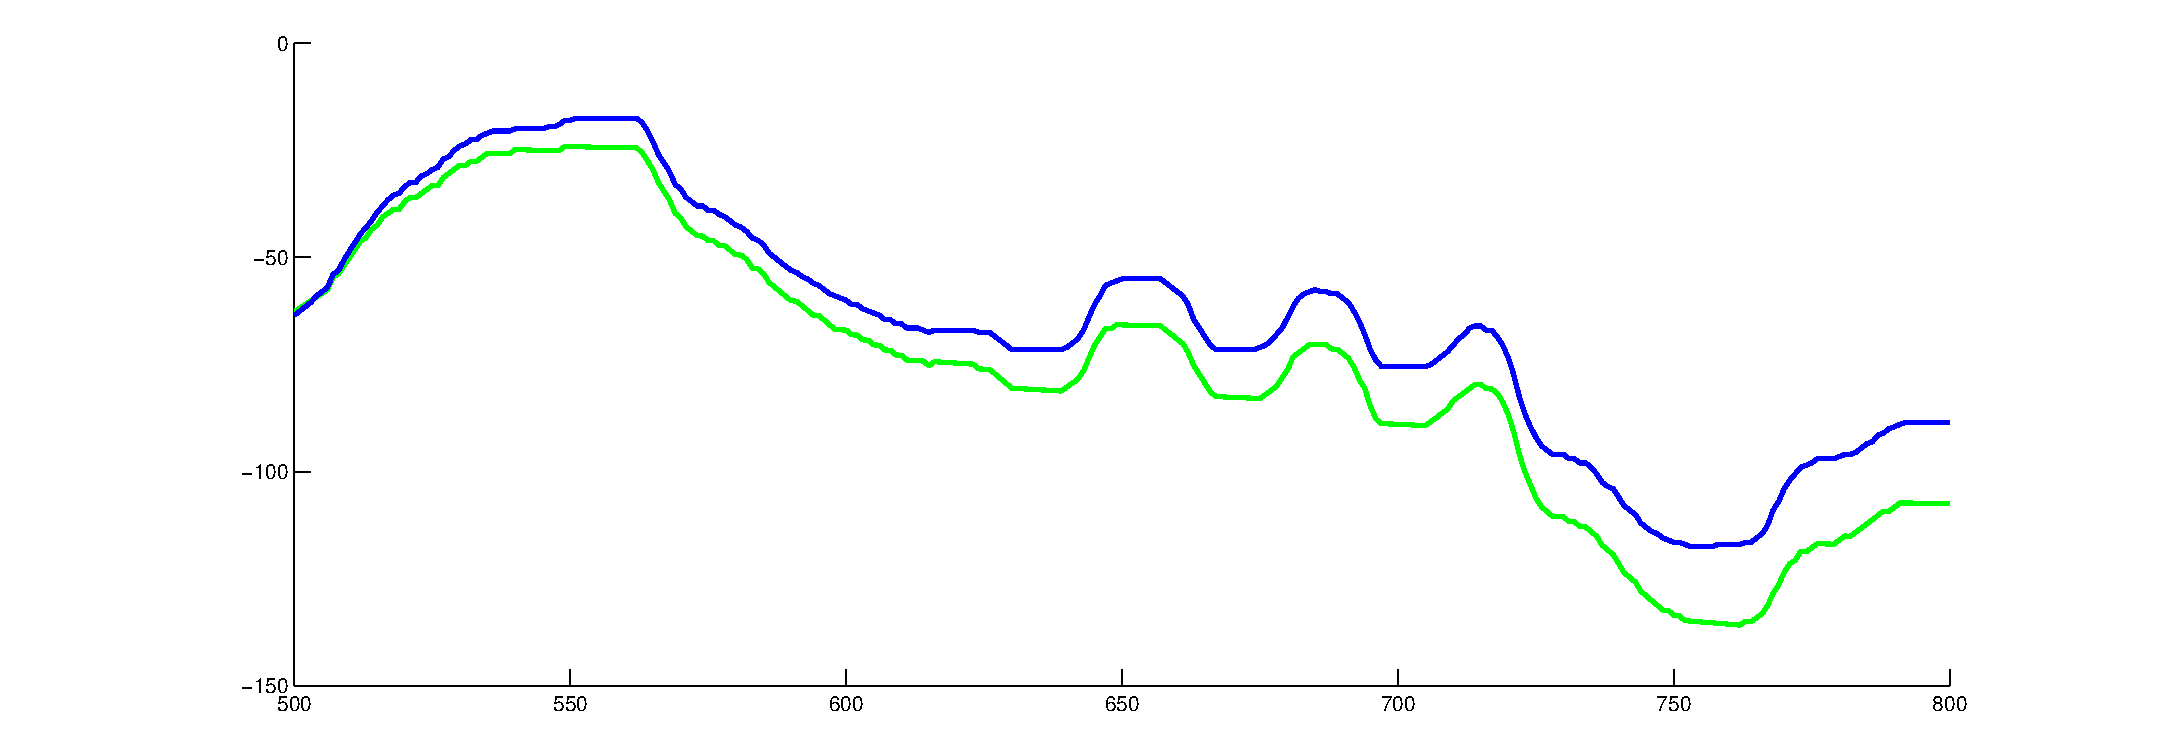
\includegraphics[width=1.0\linewidth]{images/balTacho.eps}
	\end{center}
	\caption{Bal motor fordulatszám összehasonlítása a bal és jobb motor fordulatszám átlagával}
	\label{balTachoFig}
\end{figure}

\begin{figure}[!ht]
	\begin{center}
		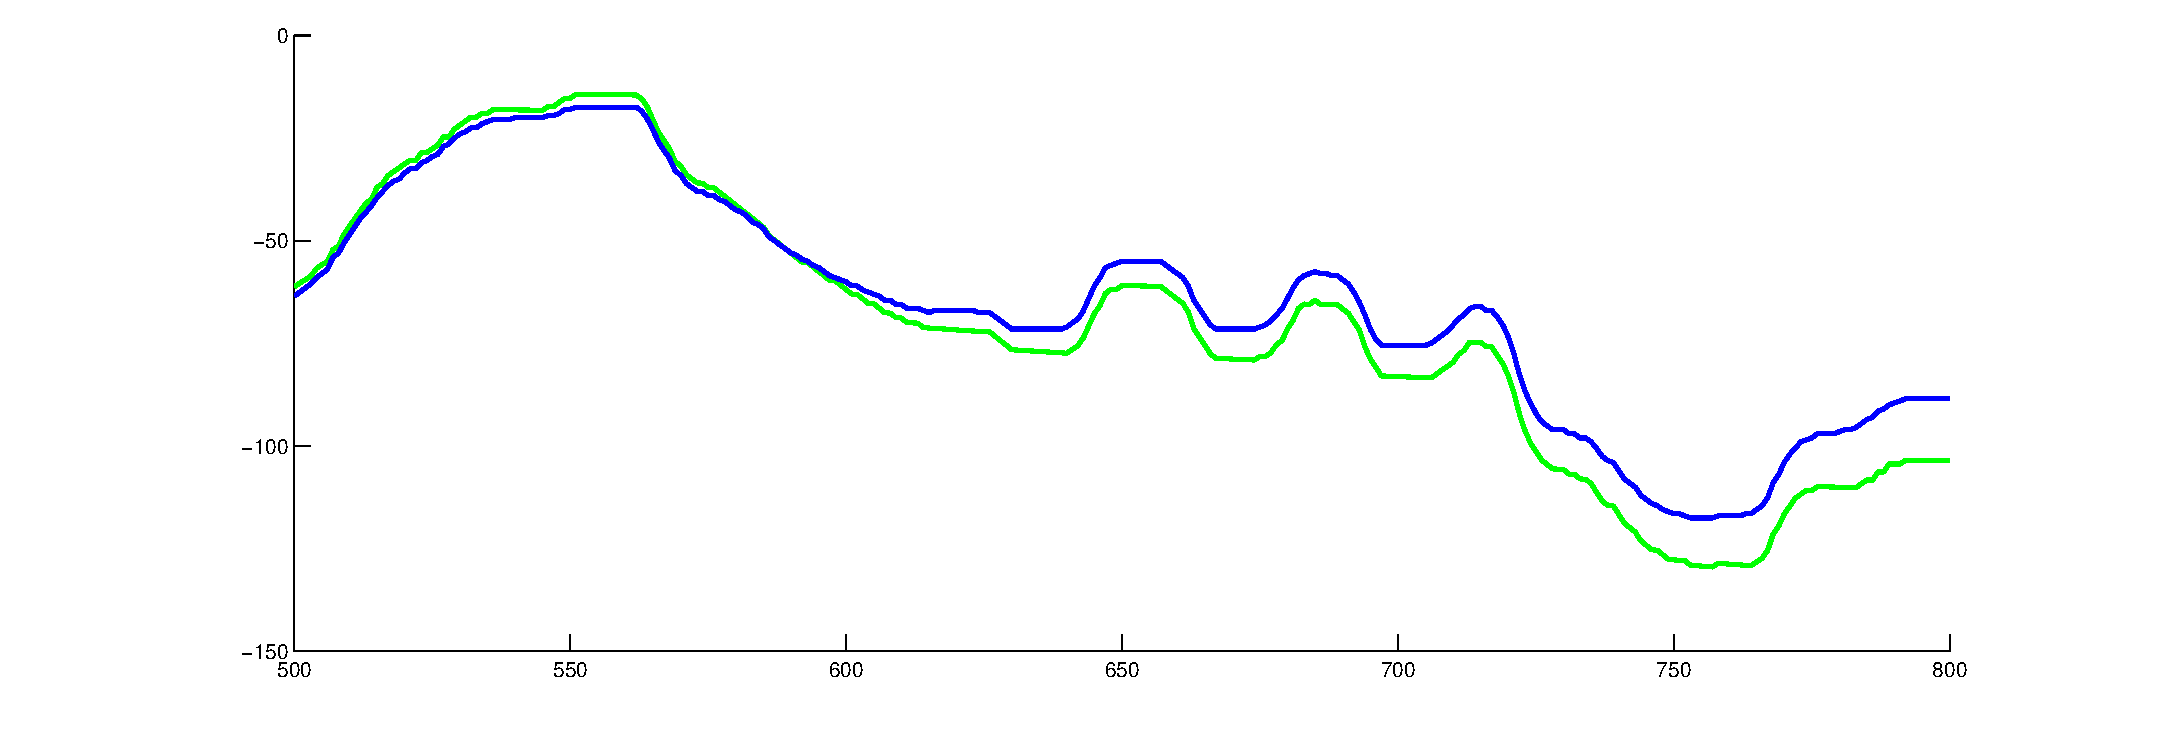
\includegraphics[width=1.0\linewidth]{images/jobbTacho.eps}
	\end{center}
	\caption{Jobb motor fordulatszám összehasonlítása a bal és jobb motor fordulatszám átlagával}
	\label{jobbTachoFig}
\end{figure}

A szinkronizálás helyességének tesztelése után, a PID szabályzó bemeneti hibáját meghatározó négy komponensnek a kiszámítását teszteltük. Az eredeti projekt szabályzó algoritmusa esetében a robot sebességének és pozíciójának kiszámításakor átlagolva volt a két motor fordulatszáma, annak érdekében, hogy kiszűrje a zajokat. Esetünkben ez módosult és elhagytuk az átlagolást. Ennek eredményeként amikor egy adott iterációban minimális különbség lépet fel a két motor fordulatszáma között akkor ez nagymértékben befolyásolta sebesség és pozíció kiszámítását. Mivel a fordulatszám különbözött ezért a sebesség és a pozíció is. E különbség iterációnként növekedett. A sebesség és a pozíció a PID bementi hibájának a két komponense ezért a kimeneti érték is különbözött, amely meghatározta a motorokra adott erő nagyságát. Tehát a motorok fordulatmérő szenzorjainak zajos mérései miatt olyan eltérés keletkezett a két motort kezelő szabályzó közt, hogy a robot elvesztette egyensúlyi állapotát.

E probléma megoldására, mivel iterációnként nőt az eltérés a két párhuzamosan futó szabályzó közt, próbáltuk súlyozni az aktuális és az azelőtti mért fordulatszámot, hogy megközelítsük az átlagolt fordulatszámot. Az így megkapott értékre számoltuk ki a robot sebességét és pozícióját. A legjobb megközelítését, amelyet az átlagolt értékkel hasonlítottunk össze az látható a \ref{balTachoFig} és a \ref{jobbTachoFig} ábrákon. A kék szín jelöli a adott motor fordulatszámát illetve a zöld jelöli a motorok az átlagolt fordulatszámot. De még ez a közelítés sem volt elegendő, hogy a robot ne veszítse el az egyensúlyát.







 
